\documentclass[12pt,a4paper,utf8x]{report}
\usepackage [frenchb]{babel}

% Pour pouvoir utiliser 
\usepackage{ucs}
\usepackage{graphicx}
\usepackage[utf8x]{inputenc}

\usepackage{url} % Pour avoir de belles url
\usepackage {geometry}

% Pour mettre du code source
\usepackage {listings}
\usepackage{verbatim}
\usepackage{fancyvrb}
% Pour pouvoir passer en paysage
\usepackage{lscape}

% Pour pouvoir faire plusieurs colonnes
\usepackage {multicol}
\usepackage{pifont}


% Pour les entetes de page
% \usepackage{fancyheadings}
%\pagestyle{fancy}
%\renewcommand{\sectionmark}[1]{\markboth{#1}{}} 
%\renewcommand{\subsectionmark}[1]{\markright{#1}} 

% Pour l'interligne de 1.5
\usepackage {setspace}
% Pour les marges de la page
\geometry{a4paper, top=2.5cm, bottom=2.5cm, left=3cm, right=2.5cm, marginparwidth=1.2cm}

\parskip=5pt %% distance entre § (paragraphe)
\sloppy %% respecter toujours la marge de droite 

% Pour les pénalités :
\interfootnotelinepenalty=150 %note de bas de page
\widowpenalty=150 %% veuves et orphelines
\clubpenalty=150 

%Pour la longueur de l'indentation des paragraphes
\setlength{\parindent}{15mm}



%%%% debut macro pour enlever le nom chapitre %%%%
\makeatletter
\def\@makechapterhead#1{%
 % \vspace*{30\p@}%
  {\parindent \z@ \raggedright \normalfont
    \interlinepenalty\@M
    \ifnum \c@secnumdepth >\m@ne
        \Huge\bfseries \thechapter\quad
    \fi
    \Huge \bfseries #1\par\nobreak
    \vskip 20\p@
  }}

\def\@makeschapterhead#1{%
%  \vspace*{30\p@}%
  {\parindent \z@ \raggedright
    \normalfont
    \interlinepenalty\@M
    \Huge \bfseries  #1\par\nobreak
    \vskip 20\p@
  }}
\makeatother
%%%% fin macro %%%%

\lstset{
basicstyle=\footnotesize,
numbers=left,
numberstyle=\normalsize,
breaklines=true,  
numbersep=7pt,
frame=single, 
}

\fvset{
frame=single,
fontsize==\footnotesize , 
numbers=left,
}

%Couverture 

\begin{document}

\begin{titlepage}

   \hfill
   \begin{center}
   \begin{minipage}[t]{12cm} 
	\huge \center Projet de Graphes, Algorithmes et Modélisation
   \end{minipage}
   \end{center}
\vfill
\begin{flushleft}
\begin{minipage}[t]{5cm}
Master 1 Informatique, \\ Aurélien Cavelan \\ Léo Rousseau
\end{minipage}
\end{flushleft}

\end{titlepage}
%\clearpage
\tableofcontents

\chapter{Compilation et Utilisation}
  \section{Compiler le Projet}
  L'archive du projet est composée de plusieurs répertoires : Un répertoire \textbf{src} qui contient les sources du projet et un
  répertoire \textbf{doc} qui contient les sources tex du présent rapport. Un makefile à la racine du projet permet de compiler les sources.

  \begin{lstlisting}
  make
  \end{lstlisting}

  \section{Utiliser le Logiciel}
  La compilation va générer un répertoir \textbf{bin} qui va contenir l'exécutable du logiciel. Pour lancer le logiciel : 
  \begin{lstlisting}
  ./bin/fleury
  \end{lstlisting}

  Le graphe à tester devra être passé au programme sur l'entré standard selon le format fixé. Après calcul sera affiché l'ordre de parcours des nœuds du graphe dans le cycle s'il existe.

  \section{Utiliser le Générateur}
  Le Projet contient également un générateur de graphes complets. Pour l'utiliser, il faut le compiler : 
  \begin{lstlisting}
  make generator
  \end{lstlisting}

  Et lui passer en paramètre $K$ le nombre de nœuds dans le graphe : 

  \begin{lstlisting}
  ./bin/generator K
  \end{lstlisting}

  Enfin, il est possible de combiner le générateur avec le lociciel afin de ne pas avoir à saisir manuellement un graphe : 

  \begin{lstlisting}
  ./bin/generator K | ./bin/fleury
  \end{lstlisting}


\chapter{Algorithme et Implémentation}
  \section{Implémentation}
    \subsection{Structure de données}
    Le projet s'appuie sur une structure de nœud deffinie de cette façon : 
    \begin{lstlisting}
struct node_t
{
    int id;
    struct node_t ** neighbours;
    int degree;
};
    \end{lstlisting} 
    Un graphe est un tableau dynamique de nœuds. Chaque nœud contient un identifiant \textbf{id}, un ensemble de voisins \textbf{neighbours} et le nombre de voisin qu'il possède : \textbf{degree}.\\ \\
    \indent Nous utilisons aussi une représentation des arêtes par couple d'entiers où chaque entier est l'identifiant d'un des nœuds.
    \begin{lstlisting}
struct edge_t {int u; int v;};
    \end{lstlisting}
    Cette structure est utilisée lors de la lecture sur l'entrée standard et la création d'un graphe. \\ \\
    \indent Nous avons aussi défini un ensemble de fonctions permettant d'utiliser un graphe comme un objet. Ces fonctions permettent nottamment la lecture, la création, la suppression et le parcour d'un graphe. Les fonctions \textbf{graph\_darken\_edge} et \textbf{graph\_undarken\_edge} servent respectivement à marquer et démarquer une arrête lors d'un parcours. Une arête marquée n'est plus visitable.

    \begin{lstlisting}
int graph_create_from_list (struct node_t * g, int n, int m, struct edge_t * e, int * count);
int graph_read_from_std (struct node_t ** gp, int * np, int * mp);
void graph_destroy (struct node_t * g, int n);
void graph_darken_edge(struct node_t * a, struct node_t * b, int x);
void graph_undarken_edge(struct node_t * a, struct node_t * b);
void graph_dfs_display (struct node_t * g, int n);
    \end{lstlisting}

    \subsection{Implémentation de l'algorithme}
L'algorithme est implémenté via la fonction \textbf{fleury} dans le fichier \textbf{main.c}. Une fois que le graphe à été lu et initialisé, cette fonction va y rechercher un cycle eulerien et, s'il existe, il sera affiché (ordre de parcours des nœuds).
 \\ \\ 
 \indent La fonction \textbf{fleury} s'appuie sur la fonction \textbf{pick\_next}. Elle sert à trouver l'identifiant du prochain nœud à visiter étant donné un nœud de départ. Pour se faire, elle effectue un parcours en profondeur \textbf{is\_not\_isthme\_dfs}. Ce test sert à vérifier qu'il existe un autre chemin entre un nœud source et un nœud destination que l'arrête qui les relie directement. Si ce test est valide, alors cela signifie que l'arrête n'est pas un isthme et peut donc être visitée (noircie). Un nouveau noeud est ajouté à la solution, sinon il faut tester les autres voisins.

  \section{Étude de Complexité}
Notre implémentation de l'algorithme cherche $m$ arêtes. À chaque fois elle peut parcourir jusqu'à $n$ voisins et pour savoir si un voisin est bon elle effectue un parcours en profondeur en O($n + m$) ; 
soit: $m * n * (m + n)$. Après développement on obient : $m^2*n+n^2*m$ or, $m>n$ donc la complexité de notre implémentation est $O(m^2*n)$. On peut observer sur la courbe ci dessous la croissance du temps d'exécution de l'algorithme (en secondes) en fonction du nombre de nœuds dans un graphe (complet). On en déduit qu'il s'agit bien d'une croissance quadratique.

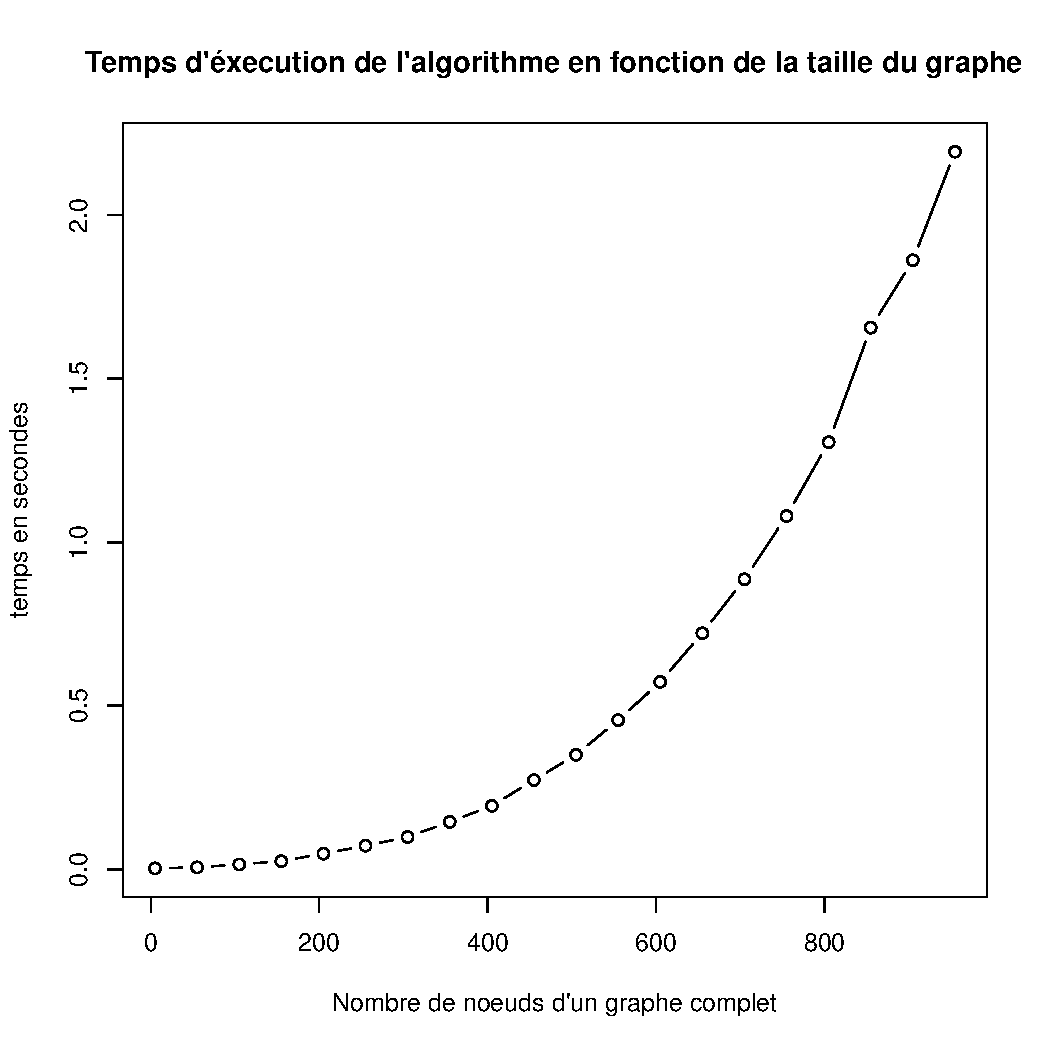
\includegraphics[scale=0.7]{img/fleury2.pdf} 
\end{document}

